%----------------------------------------------------------------------------------------
%	PACKAGES AND OTHER DOCUMENT CONFIGURATIONS
%----------------------------------------------------------------------------------------

\documentclass[twoside]{article}

\usepackage{lipsum} % Package to generate dummy text throughout this template

\usepackage[sc]{mathpazo} % Use the Palatino font
\usepackage[T1]{fontenc} % Use 8-bit encoding that has 256 glyphs
\linespread{1.05} % Line spacing - Palatino needs more space between lines
\usepackage{microtype} % Slightly tweak font spacing for aesthetics

\usepackage[hmarginratio=1:1,top=32mm,columnsep=20pt]{geometry} % Document margins
\usepackage{multicol} % Used for the two-column layout of the document
\usepackage[hang, small,labelfont=bf,up,textfont=it,up]{caption} % Custom captions under/above floats in tables or figures
\usepackage{booktabs} % Horizontal rules in tables
\usepackage{float} % Required for tables and figures in the multi-column environment - they need to be placed in specific locations with the [H] (e.g. \begin{table}[H])
\usepackage{hyperref} % For hyperlinks in the PDF

\usepackage{lettrine} % The lettrine is the first enlarged letter at the beginning of the text
\usepackage{paralist} % Used for the compactitem environment which makes bullet points with less space between them

\usepackage{abstract} % Allows abstract customization
\renewcommand{\abstractnamefont}{\normalfont\bfseries} % Set the "Abstract" text to bold
\renewcommand{\abstracttextfont}{\normalfont\small\itshape} % Set the abstract itself to small italic text

\usepackage{titlesec} % Allows customization of titles
\renewcommand\thesection{\Roman{section}} % Roman numerals for the sections
\renewcommand\thesubsection{\Roman{subsection}} % Roman numerals for subsections
\titleformat{\section}[block]{\large\scshape\centering}{\thesection.}{1em}{} % Change the look of the section titles
\titleformat{\subsection}[block]{\large}{\thesubsection.}{1em}{} % Change the look of the section titles

\usepackage{fancyhdr} % Headers and footers
\pagestyle{fancy} % All pages have headers and footers
\fancyhead{} % Blank out the default header
\fancyfoot{} % Blank out the default footer
\fancyhead[C]{ESE650 Learning in Robotics $\bullet$ March 2014 $\bullet$ Project 4} % Custom header text
\fancyfoot[RO,LE]{\thepage} % Custom footer text

\usepackage[pdftex]{graphicx}
\usepackage{epstopdf}
\usepackage{subfigure}
\usepackage{amsmath,amssymb,amsopn,amstext,amsfonts}
\usepackage{url}
\usepackage[usenames,dvipsnames]{color}
\usepackage{siunitx}
\usepackage{amsmath}
\usepackage{amsfonts}
\usepackage{amssymb}

\graphicspath{{fig/}}
\newcommand{\W}{\mathcal{W}}
\newcommand{\X}{\mathcal{X}}
\newcommand{\Y}{\mathcal{Y}}
\newcommand{\Z}{\mathcal{Z}}
\newcommand{\red}[1]{\textcolor{red}{#1}}
\newcommand{\brown}[1]{\textcolor{brown}{#1}}
%----------------------------------------------------------------------------------------
%	TITLE SECTION
%----------------------------------------------------------------------------------------

\title{\vspace{-15mm}\fontsize{24pt}{10pt}\selectfont\textbf{Localization and Mapping}} % Article title

\author{
\large
\textsc{Chao Qu}\thanks{A thank you or further information}\\[2mm] % Your name
\normalsize University of Pennsylvania \\ % Your institution
\normalsize \href{mailto:quchao@seas.upenn.edu}{quchao@seas.upenn.edu} % Your email address
\vspace{-5mm}
}
\date{}

%----------------------------------------------------------------------------------------

\usepackage{graphicx}
\begin{document}


\maketitle % Insert title

\thispagestyle{fancy} % All pages have headers and footers

%----------------------------------------------------------------------------------------
%	ABSTRACT
%----------------------------------------------------------------------------------------

%\begin{abstract}
%
%\noindent Hey, I'm just an abstract. % Dummy abstract text
%
%\end{abstract}

%----------------------------------------------------------------------------------------
%	ARTICLE CONTENTS
%----------------------------------------------------------------------------------------

%----------------------------------------------------------------------------------------
%	INTRODUCTION
%----------------------------------------------------------------------------------------

\begin{multicols}{2} % Two-column layout throughout the main article text

\section{Introduction}
\lettrine[nindent=0em,lines=2]{D}ue to lack of time, this report will be relatively short
and concise compared to my previous reports.

%----------------------------------------------------------------------------------------
%	PRE-PROCESSING
%----------------------------------------------------------------------------------------

\section{Pre-processing}
The pre-processing step is basically the same as that of project 2. Mainly converting raw
imu reading to physical unit. For laser data, I select range readings subject to distance
and angle restriction.

%----------------------------------------------------------------------------------------
%	METHODS
%----------------------------------------------------------------------------------------

\section{Methods}
\subsection{Motion Model}
For motion model, I refer to the one in Thrun's \textit{Probabilistic Robotics} with a few
modifications. The model is shown as follows:
\begin{align*}
dR &= \mbox{average encoder right} \\
dL &= \mbox{average encoder left} \\
dC &= \frac{dR + dL}{2} \\
\alpha &= \frac{dR-dL}{w_{eff}} \\
x_{t+1} &= x_{t} + \cos(\theta + \alpha/2) \\
y_{t+1} &= y_{t} + \sin(\theta + \alpha/2) \\
\theta_{t+1} &= \theta_t + \alpha
\end{align*}

For localization and mapping, I use the MCL algorithm, which is also from Thrun's work.
A brief description of the algorithm is shown as follows:
\begin{enumerate}
\item initialize number of particles $m$
\item sample $m$ particles from motion model
\item use measurement model to weight each particle
\item re-sample based on number of effective particles
\item assign new particles and iterate again
\end{enumerate}
%----------------------------------------------------------------------------------------
%	RESULTS
%----------------------------------------------------------------------------------------

\section{Results}
Here are some of the results on training set
\begin{figure}[H]
\centering
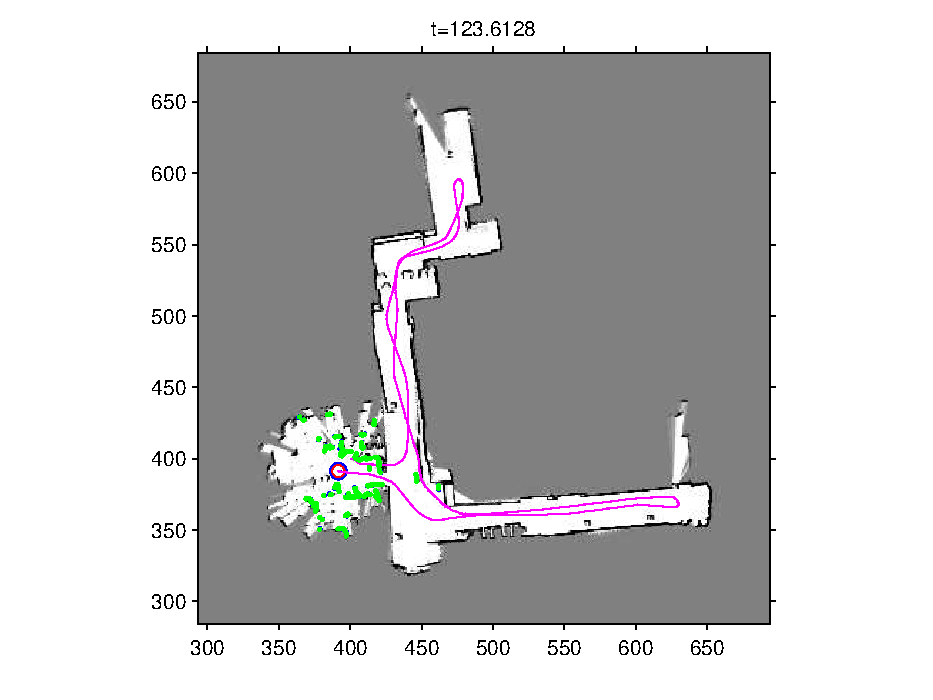
\includegraphics[width=\columnwidth]{fig/map20.pdf}
\caption{Map 20}
\label{fig:map20}
\end{figure}

\begin{figure}[H]
\centering
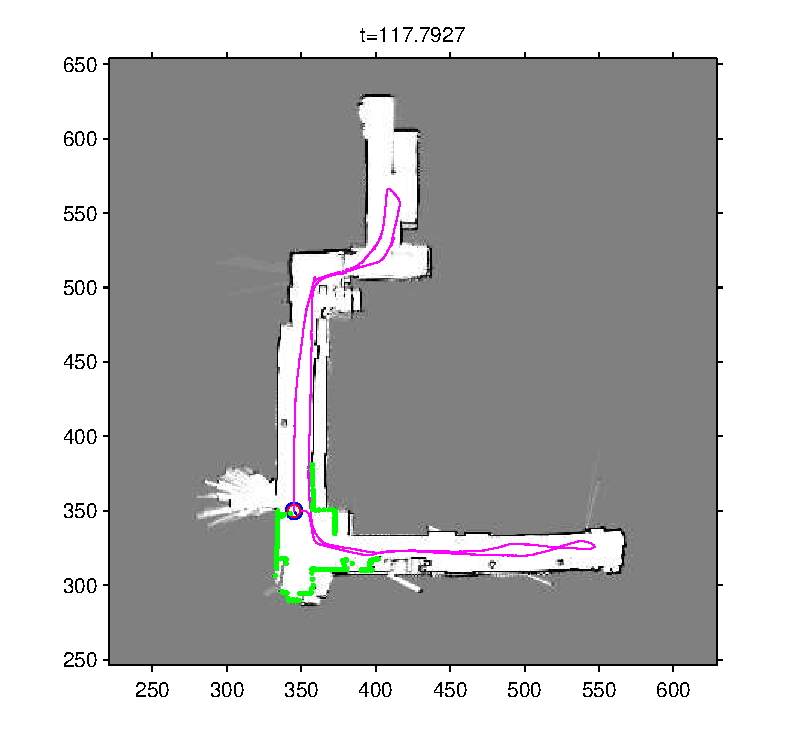
\includegraphics[width=\columnwidth]{fig/map21.pdf}
\caption{Map 21}
\label{fig:map21}
\end{figure}

\begin{figure}[H]
\centering
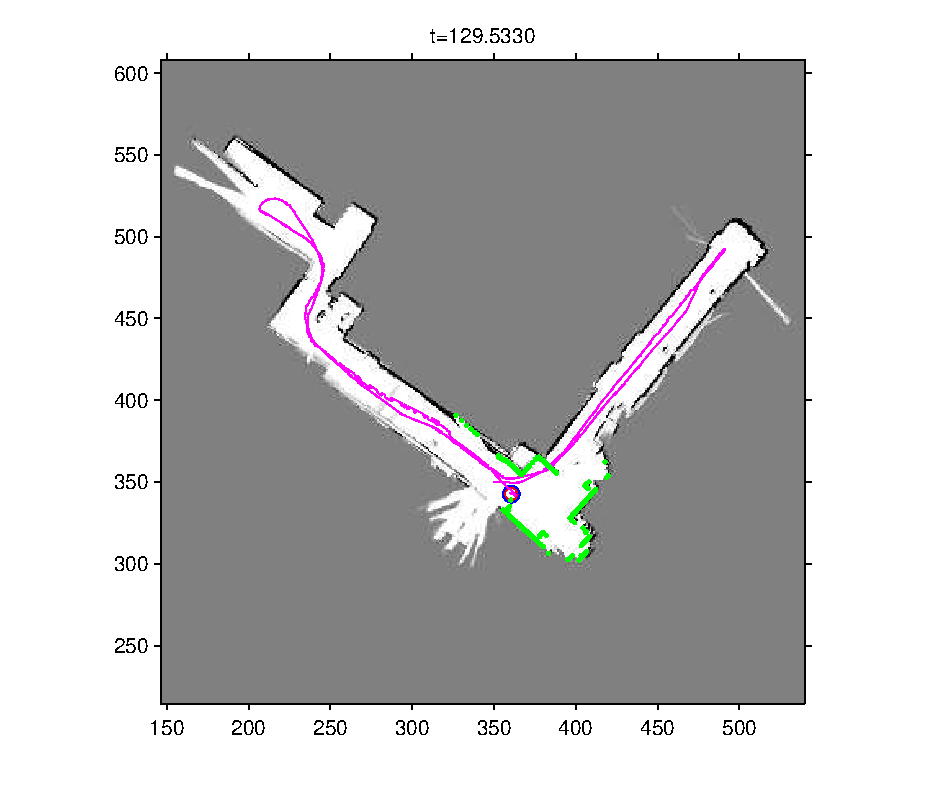
\includegraphics[width=\columnwidth]{fig/map22.pdf}
\caption{Map 22}
\label{fig:map22}
\end{figure}

\begin{figure}[H]
\centering
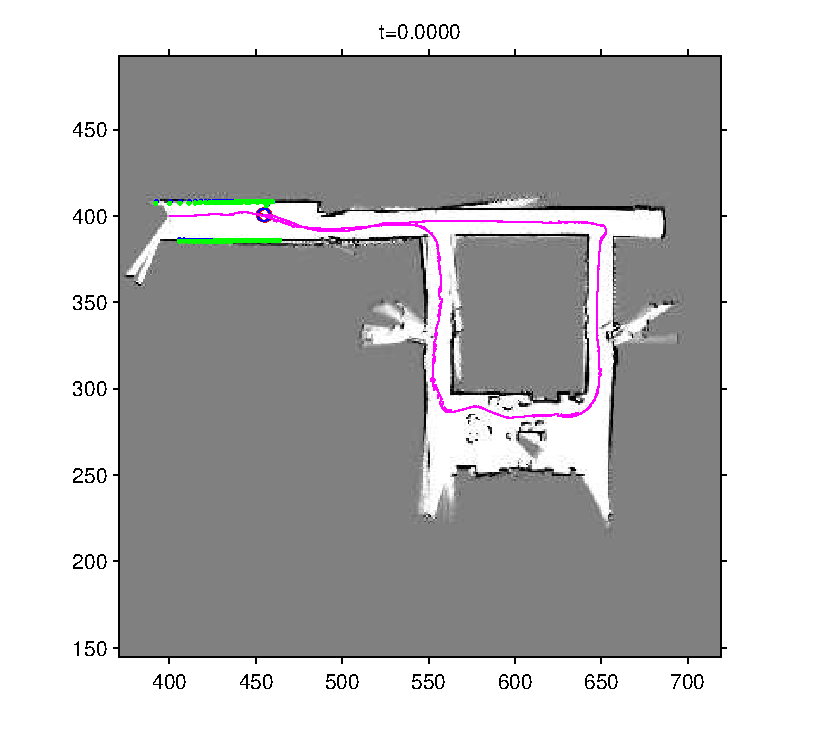
\includegraphics[width=\columnwidth]{fig/map23.pdf}
\caption{Map 23}
\label{fig:map23}
\end{figure}

\begin{figure}[H]
\centering
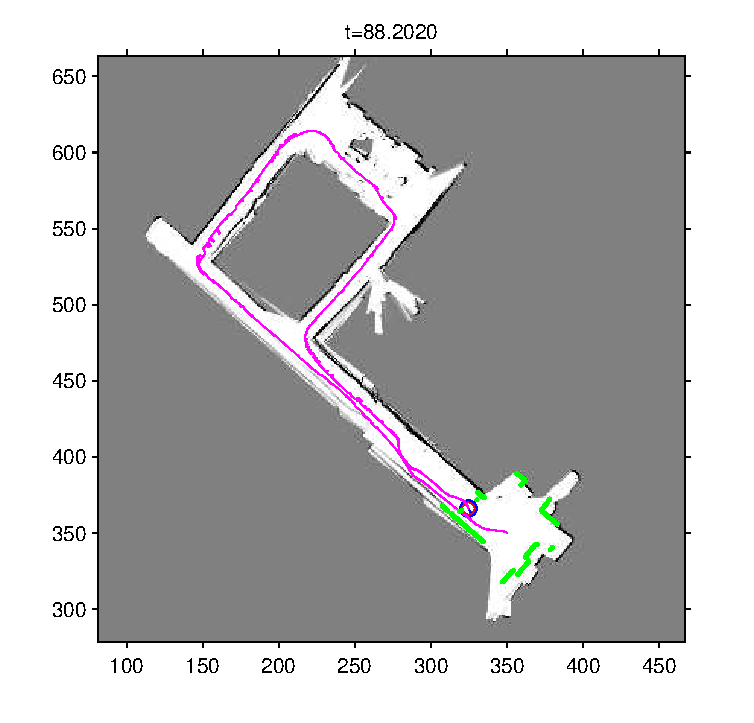
\includegraphics[width=\columnwidth]{fig/map24.pdf}
\caption{Map 24}
\label{fig:map24}
\end{figure}

\begin{figure}[H]
\centering
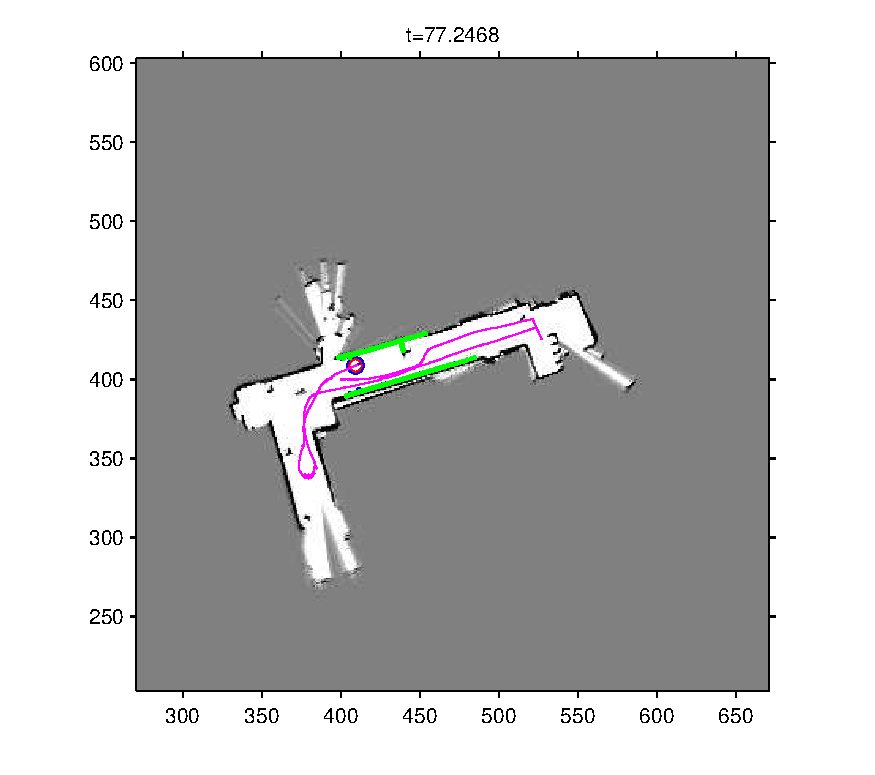
\includegraphics[width=\columnwidth]{fig/test1.pdf}
\caption{Test 1}
\label{fig:test1}
\end{figure}

\begin{figure}[H]
\centering
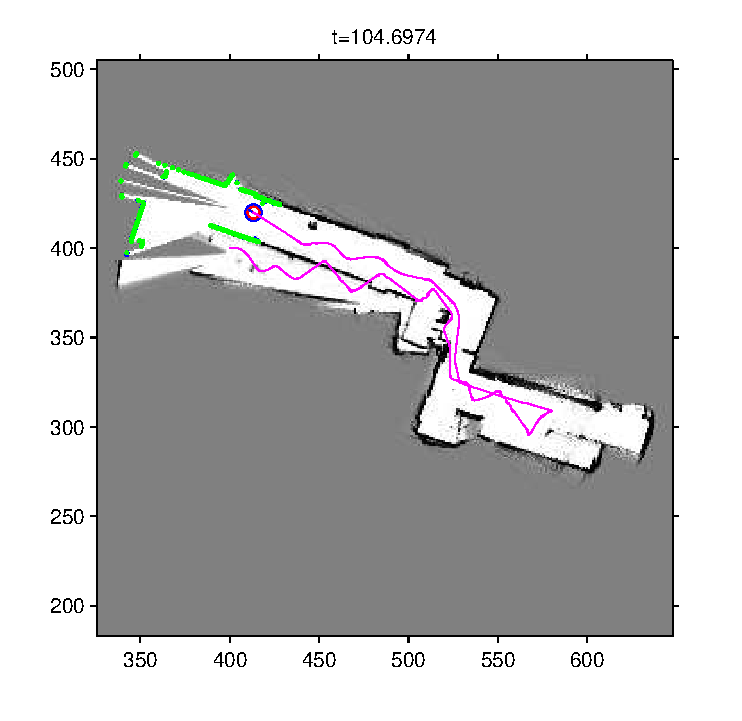
\includegraphics[width=\columnwidth]{fig/test2.pdf}
\caption{Test 2}
\label{fig:test2}
\end{figure}
%----------------------------------------------------------------------------------------
%	DISCUSSION
%----------------------------------------------------------------------------------------

\section{Discussion}
I wasted most of my time on debugging my code until I found out that in testMapCorrelation,
the example uses ceil for getting cell indices, while in map\_correlation, it uses round.
This type of inconsistency caused my correction to have a constant rotation in it. I found this
out 2 hours before the class, and now it seems to work reasonably.
%----------------------------------------------------------------------------------------
%	REFERENCE LIST
%----------------------------------------------------------------------------------------

%\begin{thebibliography}{2} % Bibliography - this is intentionally simple in this template
%
%\bibitem{Vesa00}
%Vesa-Matti Mantyla, \emph{Hand gesture recognition of a mobile device user}. Multimedia and Expo, 2000. ICME 2000.
%
%\bibitem{Elmez07}
%Elmezain M. and Al-Hamadi A., \emph{A Hidden Markov Model-based continuous gesture recognition system for hand motion trajectory}. 19th International Conference on Pattern Recognition, ICPR 2008.
%
%\bibitem{Rabiner89}
%Lawrence R. Rabiner, \emph{A Tutorial on Hidden Markov Models and Selected Applications in Speech Recognition}. Proceedings of the IEEE, 1989.
%
%\end{thebibliography}

%----------------------------------------------------------------------------------------

\end{multicols}
\end{document}
